\subsection{Model architecture}

\begin{figure}[h]
    \begin{minipage}{0.68\linewidth}
    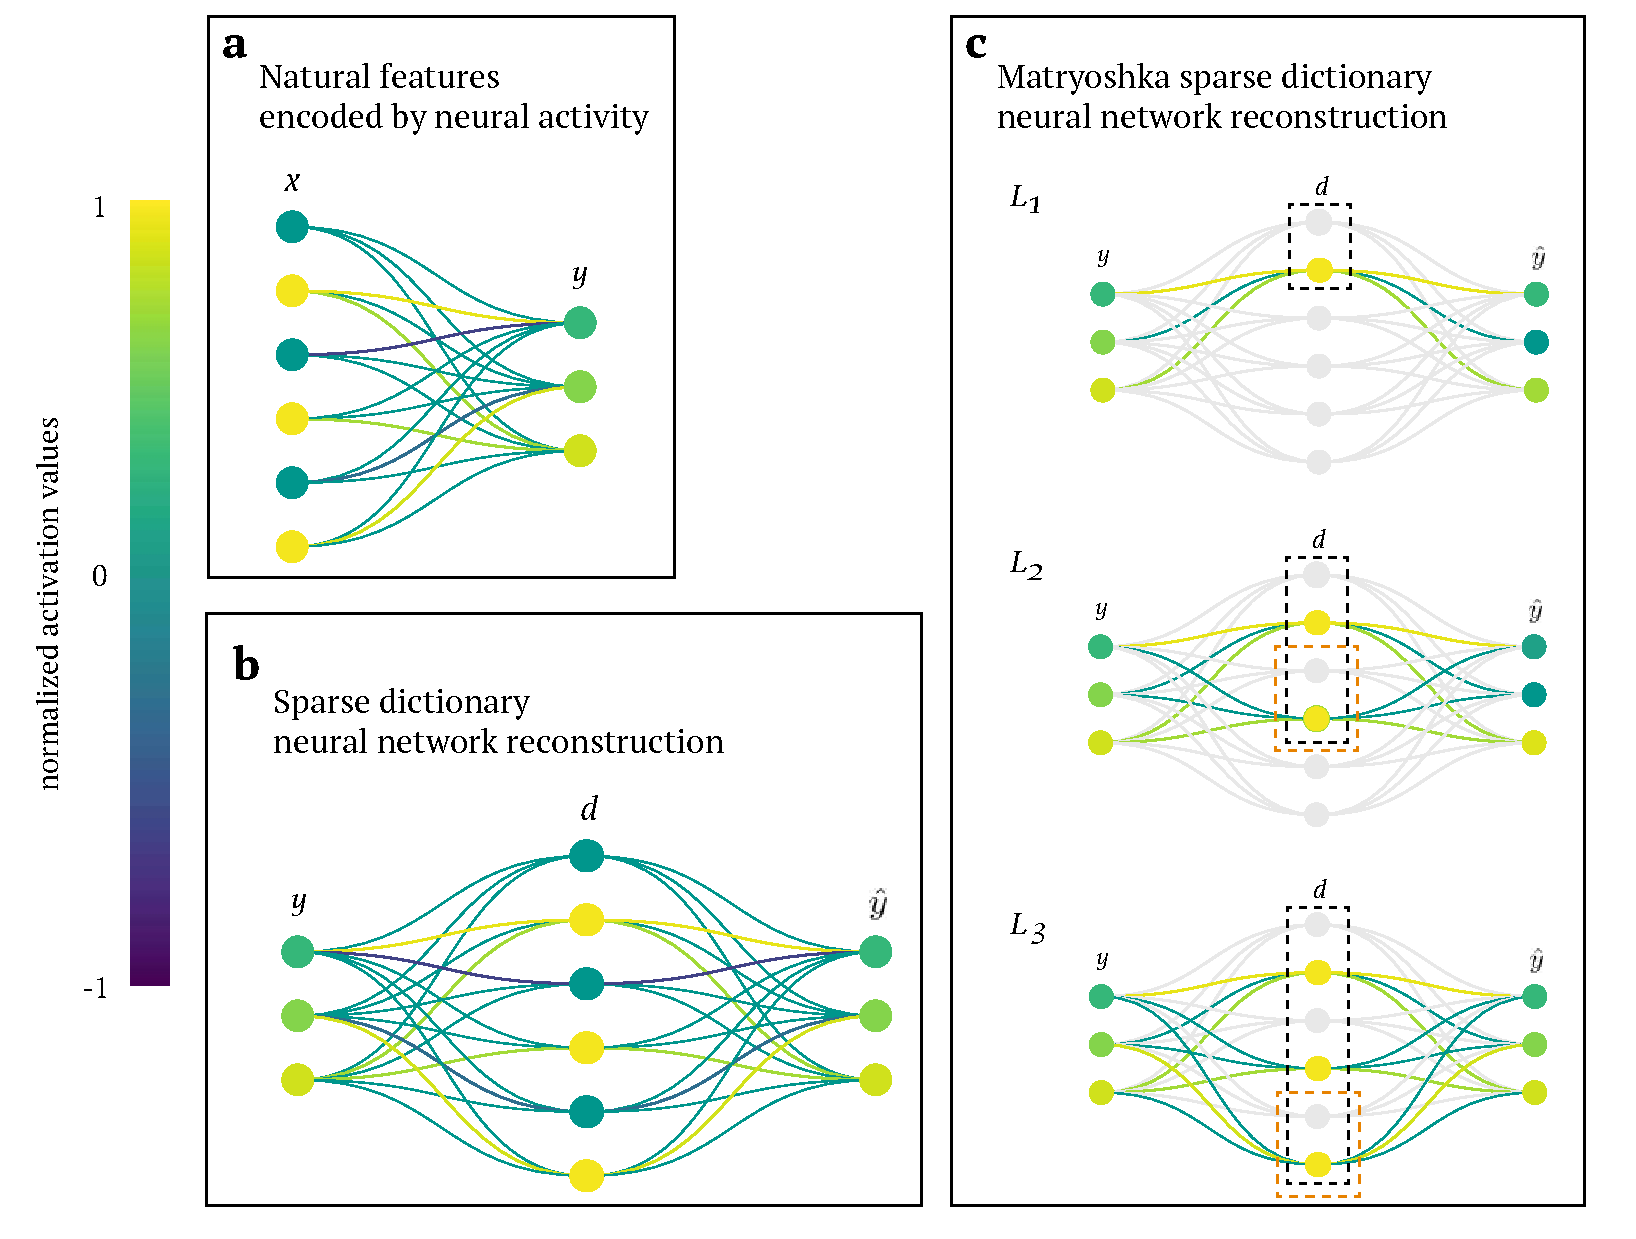
\includegraphics[width=\linewidth]{figures/sdnn_arch.pdf}
    \end{minipage}%
    \begin{minipage}{0.33\linewidth}
    \caption{
        \textbf{MINI's sparse dictionary neural network architecture.} \\
        \small (\textbf{a}) Natural features $x$ get encoded by neural activity $y$. (\textbf{b}) A sparse dictionary neural network attempts to recreate neural activity $\hat{y}$ from $y$. If $\hat{y}$ tries to recreate $y$ exactly, then the model is an autoencoder, while in other situations it may be a transcoder or crosscoder. ()\textbf{c}) A Matryoshka spare dictionary neural network segments the latent space into multiple levels, each of which attempts to do a full reconstruction of the target neural activity. In this case, latents exclusive to the highest-level will often correspond to high-level features (e.g. a round object), while latents exclusive to the lowest-level will often correspond to low-level features (e.g. a basketball).
    }
    \label{fig:sdnn_arch}
    \end{minipage}
\end{figure}

\begin{itemize}
    \item Usefulness of SDL methods in Mech interp.
    
    \item Variant of MSAE as variant of SAE.
    \begin{itemize}
        \item Briefly mention other archs tried: batchTopK winner for sparsity enforcement.
    \end{itemize}
    
    \item In addition to MSAE levels width, briefly mention hyperparameters, expound in Appendix.
    \begin{itemize}
        \item topk per level, loss X per level, seq len for neural data, seq len for latent space used with transformer layer in decoder
    \end{itemize}
    
    \item Show latex formulas for encoder, decoder, total loss.
\end{itemize}